\documentclass[11pt]{article}
\usepackage{graphicx}
\graphicspath{ {./images/} }

\usepackage{algorithm}
\usepackage{algpseudocode}
\usepackage{hyperref}

\usepackage{sectsty}
\usepackage{graphicx}
\usepackage[font=small,labelfont=bf]{caption} % Required for specifying captions to tables and figures

% Margins
\topmargin=-0.45in
\evensidemargin=0in
\oddsidemargin=0in
\textwidth=6.5in
\textheight=9.0in
\headsep=0.25in

\title{ %

\includegraphics[width=0.4\textwidth]{UniCT-Logo-Nero}~\\
A solution for MWVC using Iterated Local Search \\ 
\large Laboratorio Intelligenza Artificiale (LM-18) \\ Università degli Studi di Catania - A.A 2021/2022 \\
}
\author{ Danilo Leocata \\ Docente: Mario Pavone}
\date{\today}

\begin{document}

\maketitle	
\pagebreak

% Optional TOC
% \tableofcontents
% \pagebreak

%--Paper--

\section{Introduzione}

Si propone una soluzione per il Weight Vertex Cover problem utilizzando l'Iterated Local Search: l'obbiettivo proposto è trovare la migliore soluzione, data un istanza, con il minimo numero di iterazioni. Il codice è disponibile al \href{https://github.com/khalld/mwvc-using-ils}{seguente} repository di GitHub. \\
Prima di procedere con l'implementazione e la scelta dell'algoritmo, sono state consultate e prese in considerazioni varie pubblicazioni riguardanti la soluzione del problema (indicate a fine relazione). È stata trovata sin da subito interessante implementare una soluzione utilizzando l'Iterated Local Search, in particolare se ne propone una versione che perserva soluzioni non ottime sfruttando un \textit{term memory}.

Sfruttando l'ILS, è possibile ottenere sin da subito una soluzione \textit{completa} (intesa quando l'insieme dei nodi selezionati permette di raggiungere tutti i nodi dell'istanza) dopo poche iterazioni e migliorarla. Inoltre, sfruttando il \textit{term-memory} è possibile tenere traccia delle migliori soluzioni trovate permettendo di accettare e continuare la ricerca su soluzioni peggiori senza perderne traccia avendo la possibilità di ripescarle nell'operatore di perturbazione.

\pagebreak
\section{Primo approccio}

Le informazioni delle istanze dal file \verb|.txt| sono state estratte per mezzo della classe \verb|CustomGraph|.
È stata importata ed utilizzata la libreria \verb|NetworkX| per visualizzare graficamente le istanze come reti. Una demo del notebook Jupiter è disponibile \href{https://github.com/khalld/mwvc-using-ils/blob/main/visualize-instances.ipynb}{qui}

\begin{center}
\begin{minipage}{0.48\linewidth}
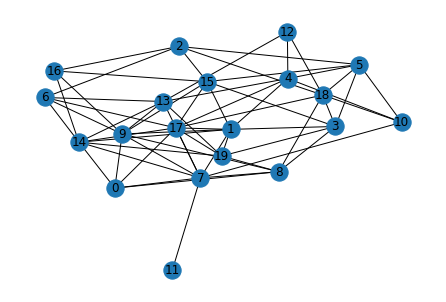
\includegraphics[width=\linewidth]{output_1}
\end{minipage}%
\begin{minipage}{0.49\linewidth}
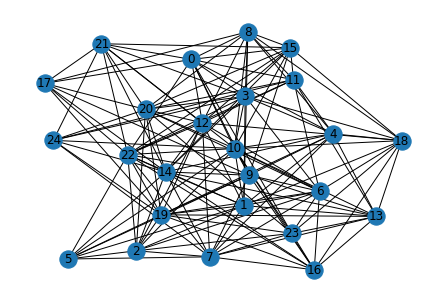
\includegraphics[width=\linewidth]{output_2}
\end{minipage}
\begin{minipage}{0.49\linewidth}
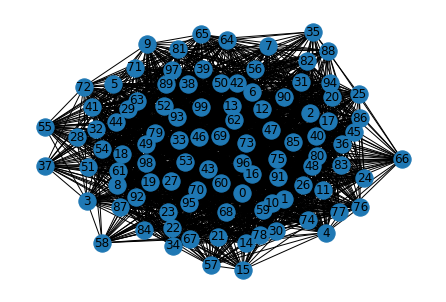
\includegraphics[width=\linewidth]{output_3}
\end{minipage}
\captionof{figure}{Visualizzazione grafica delle istanze fornite}
\end{center}

Utilizzando l'apposita funzione di conversione \verb|cnv_txt_instance|, saranno estratti dall'istanza rispettivamente:
\begin{itemize}
\item{i nodi con il relativo peso e vicinato;}
\item{numero totale di nodi presenti in un'istanza.}
\end{itemize}

\pagebreak

\section{ILS}

Sono stati testati sulle istanze due tipi di approcci:

\begin{itemize}
\item{costruzione di una soluzione a partire da un nodo iniziale scelto randomicamente;}
\item {scoperta della soluzione migliore partendo dalla soluzione peggiore (intesa così quella che ha selezionati tutti i nodi presenti nell'istanza);}
\end{itemize}

Il primo approccio è stato scartato durante la fase di test in quanto molto lento rispetto all'altro, principalmente con istanze MPI/LPI. È stato preso in considerazione, ma scartato durante la fase di test, il random restart della soluzione dato che non ha portato migliorie al risultato finale.
Nel dettaglio, l'algoritmo ILS presentato parte dalla soluzione \textit{peggiore}, con tutti i nodi dell'istanza selezionati, e per mezzo dell'operatore di perturbazione e della local search si cercherà di ottimizzare la soluzione.

\begin{algorithm}
\caption{\texttt{Iterated Local Search}}
\begin{algorithmic}
    \Require {\texttt{list of all nodes of instances}}

\State {\texttt{CurrentSolution = Solution with all available nodes selecte}d}
\State {\texttt{initialize an empty term-memory}}
\While{ \texttt{max evaluations} }   

    \State {\texttt{SolutionToChange = CurrentSolution} }
    \State {\texttt{apply Perturbation to SolutionToChange} }
    \State {\texttt{apply LocalSearch to SolutionToChange} }
    \State{
        \If{\texttt{cost of SolutionToChange < cost of CurrentSolution and SolutionToChange not in term-memory}}
        \State {\texttt{add SolutionToChange in term-memory}}
        \EndIf
    }
    \State {\texttt{CurrentSolution = SelectCriteria(CurrentSolution, SolutionToChange, term-memory)}}
\EndWhile
\Return { \texttt{CurrentSolution}}
\end{algorithmic}
\end{algorithm}

\pagebreak

\section{Operatore di perturbazione}

L'idea generale della perturbazione è quella di modificare i parametri ad ogni iterazione applicando una perturbazione sui nodi selezionati dalla soluzione.
Un buon algoritmo deve evitare di far cadere sempre nello stesso minimo locale, di conseguenza si è optato per rimuovere un singolo nodo alla soluzione data.

Sono stati proposte delle varianti, gli pseudocodici sono i seguenti:

\begin{algorithm}
\caption{Perturbation - A}
\begin{algorithmic}
\Require{ \texttt{Solution} }
\State{\texttt{add random node from list of unselected}}
\State{\texttt{remove random node from list of already selected}}
\State{\Return{\texttt{solution}}}
\end{algorithmic}
\end{algorithm}


\begin{algorithm}
    \caption{Perturbation - B}
    \begin{algorithmic}
    \Require{ \texttt{Solution} }
    \State{\texttt{random perturbation  = get random number from (1, length of selected nodes / 2)}}
    
    \For{\texttt{i in range(0, random perturbation)}}
        \State \texttt{
            remove random node from already selected nodes
        }
        \State \texttt{
            add random node from unselected list
        }
    \EndFor
    
    \Return {\texttt{perturbed solution}}
\end{algorithmic}
\end{algorithm}


\begin{algorithm}
    \caption{Perturbation - C}
    \begin{algorithmic}
    \Require{ \texttt{Solution} }
    \State{\texttt{pert nds remv = get random number from (1, length of selected nodes / 2)}}
    \State{\texttt{pert nds add = get random number from (1, 2)}}

    \For{\texttt{i in range(0, perturbed removed nodes)}}
        \State \texttt{
            remove random node from already selected nodes
        }
    \EndFor
    \If{
        \texttt{ perturbed solution has unreached nodes}
    }
        \For{\texttt{i in range(0, perturbed added nodes)}}
            \State \texttt{
                add random node from unselected nodes list
            }
        \EndFor
    \EndIf
    \Return {\texttt{perturbed solution}}
\end{algorithmic}
\end{algorithm}


In particolare la versione \texttt{C} è stata pensata per le istanze LPI. Inoltre, tra le migliorie che la perturbazione potrebbe apportare alla soluzione vi è:
\begin{itemize}
\item{l'eliminazione automaticamente di cicli se questa contiene dei nodi ridondanti;}
\item{potrebbe rendere la soluzione non completa: di conseguenza applicando nuovamente la LocalSearch è possibile trovare un nodo candidato migliore rispetto a quello rimosso.}
\end{itemize}

Sono stati testati su un insieme di istanze ridotte, utilizzando \verb|SelectBestCandidateWeight| come criterio di selezione, spiegato nel dettaglio successivamente.

\begin{center}
    TODO INSERISCI TABELLA O quattro grafici ......
\end{center}

Dati i risultati dunque si è deciso di calcolare i benchmark di tutte le istanze con operatore di perturbazione... TODO

\pagebreak

\section{Local Search e criterio di selezione del nodo migliore}

Una delle difficoltà trovate durante l'implementazione è stata la determinazione del criterio di selezione del nodo nella $LocalSearch$ di cui è stato trovato opportuno implementarne una versione generica, in modo tale da avere la possibilità di cambiare il criterio facilmente.

\begin{algorithm}
\caption{LocalSearch}
\begin{algorithmic}
\Require{ \texttt{Solution, BestCandidateCriterio}}

\While{
    \texttt{solution is complete}
}
    \State {\texttt{best candidate = BestCandidateCriterio()}}
    \State {\texttt{add best candidate to solution}}
\EndWhile
\State \Return solution
\end{algorithmic}
\end{algorithm}

Volendo ottimizzare il tempo di esecuzione, dopo numerosi test, è stato trovato opportuno procedere con una ricerca First Improvement: durante la prima fase è stata implementata la Random Selection che funziona piuttosto bene su istanze piccole, ma al crescere del numero di nodi da esplorare peggiora. Mentre non è stato considerato vantaggioso effettuare una esplorazione su tutti i nodi prima di effettuare la scelta (best improvement).

Generalmente, un nodo può essere più propenso ad essere aggiunto alla soluzione in base al:
\begin{itemize}
    \item {peso;}
    \item {numero di nodi vicini: 'pagare' il costo di un nodo più costoso ma con un elevato numero vi vicini, potrebbe essere più efficiente che selezionare nodi con costo inferiore da cui si otterrà lo stesso vicinato}
\end{itemize}

Sono state implementate delle metriche per valutare il miglior nodo da inserire all'interno della soluzione data una lista di nodi candidati:

\begin{algorithm}
\caption{\texttt{SelectBestCandidateRandomly}}
\begin{algorithmic}
    \Require {\texttt{list of nodes}}
    \State {\texttt{sort list of nodes (randomly) by lower weight or major number of neighbors}}
    \State \Return {\texttt{first element of ordered list}}
\end{algorithmic}
\end{algorithm}

\begin{algorithm}
\caption{\texttt{SelectBestCandidateWeight}}
\begin{algorithmic}
    \Require {\texttt{list of nodes}}
    \State {\texttt{sort list of nodes by lower weight}}
    \State {\texttt{\Return first element of ordered list}}
\end{algorithmic}
\end{algorithm}

\begin{algorithm}
\caption{\texttt{SelectBestCandidateNeighborhood}}
\begin{algorithmic}
    \Require \texttt{list of nodes}
    \State \texttt{sort list of nodes by higher number of nodes}
    \State \Return \texttt{first element of ordered list}
\end{algorithmic}
\end{algorithm}

\pagebreak

\section{Criterio di accettazione}

L'utilizzo del term memory permette di 'accettare' soluzioni peggiori rispetto ad altre e continuare la ricerca senza perder traccia di tutte le soluzioni trovate.
In sintesi, se la soluzione perturbata è simile alla corrente il criterio di accettazione può ripescare, randomicamente una delle soluzioni presenti nel \verb|term-memory| e continuare la ricerca.


\begin{algorithm}
\caption{\texttt{Acceptance criteria}}
\begin{algorithmic}
    \Require \texttt{current solution, perturbed solution, term memory}
    \State \texttt{prob1 = get random number from 0 to 5}

    \If{ \texttt{ prob1 mod 2 == 0} }
        \If{ \texttt{ term-memory has at least 2 element}}
            \State \texttt{prob2 = get random number from 0 to 1}
            \If{ \texttt{ prob2 == 0} }
                \Return \texttt{ select one randomly in term memory}
            \Else{ \Return \texttt{ solution with less cost in term-memory} }
            \EndIf
        \EndIf
    \Else{
        \If{ \texttt{cost of perturbed solution < cost of current solution} }
        \Return \texttt{perturbed solution}
        \EndIf
    }
    \EndIf
    \State \Return \texttt{random choice between (perturbed solution, current solution)}
\end{algorithmic}
\end{algorithm}

\pagebreak

\section{Benchmarks e conclusione}

È stato implementato uno script che permette di salvare i benchmark le soluzioni ottenute dalle istanze su  file \verb|.xls|.
La tabella riassuntiva dei benchmarks delle quattro varianti di ILS è consultabile al \href{https://github.com/khalld/mwvc-using-ils/tree/main/benchmarks}{seguente} link). È stato inoltre implementato un metodo per visualizzare i grafici di convergenza dell'algoritmo sulle istanze utilizzando \verb|matplotlib|. (ne saranno importati solo alcuni per alleggerire la repository)

\begin{center}
\begin{minipage}{0.48\linewidth}
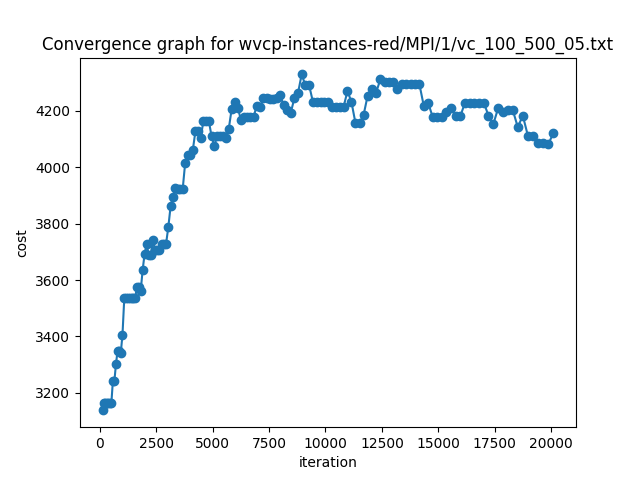
\includegraphics[width=\linewidth]{conv_graph_vc_100_500_05_rand_A.png}
\end{minipage}%
\begin{minipage}{0.49\linewidth}
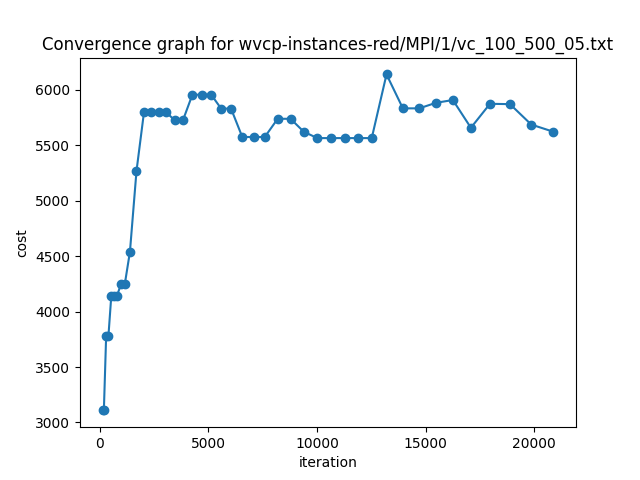
\includegraphics[width=\linewidth]{conv_graph_vc_100_500_05_rand_B.png}
\end{minipage}
\begin{minipage}{0.49\linewidth}
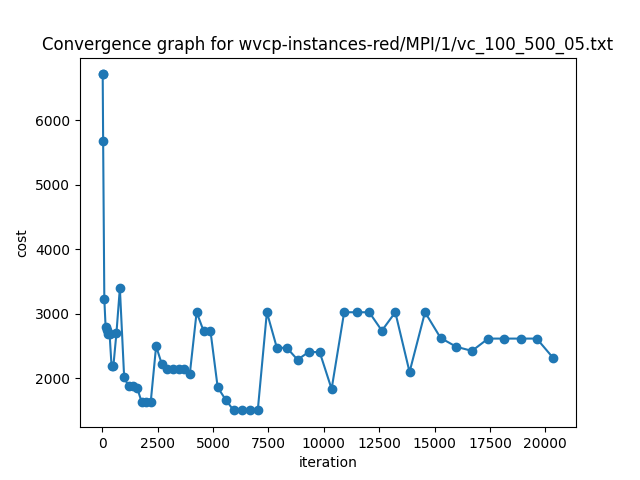
\includegraphics[width=\linewidth]{conv_graph_vc_100_500_05_rand_C.png}
\end{minipage}
\begin{minipage}{0.49\linewidth}
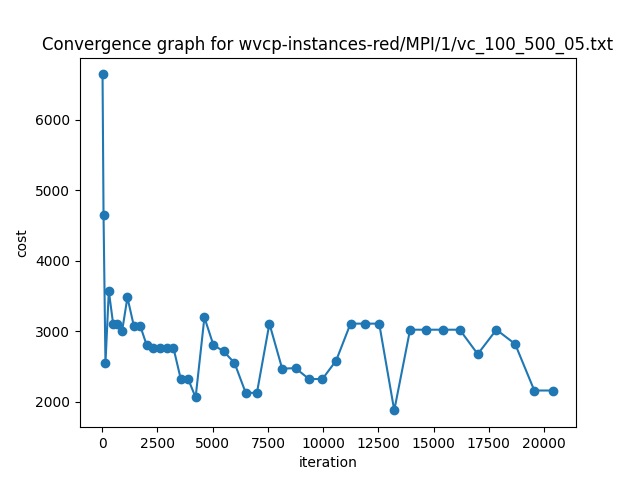
\includegraphics[width=\linewidth]{conv_graph_vc_100_500_05_rand_D.png}
\end{minipage}
\captionof{figure}{Sample grafici di convergenza delle quattro varianti di ILS su istanza}
\end{center}

\pagebreak

Guardando i grafici di convergenza e , si deduce che le ultime due versioni presentate performano meglio rispetto alle ultime due: in particolare \verb|ILS versione D| sembrerebbe performare meglio rispetto ad \verb|ILS versione C| nonostante in alcuni casi i valori della soluzione finale trovati siano peggiori.
\textbf{Si nota inoltre che eliminare dal grafico di convergenza le prime su alcune soluzioni trovate su istanze SPI ed MPI ne renderebbe più agevole la visualizzazione.}

Quest'ultimo è stato eseguito, su tutte le istanze con i tre criteri di selezione del candidato elencati precedenemente. 
I risultati migliori sono stati ottenuti con \verb|SelectBestCandidateWeight|.

\begin{table}[!ht]
    \centering
    \begin{tabular}{|l|l|l|l|}
    \hline
        Instance txt & Worst solution & Best solution cost & Mean evaluations for each sol \\ \hline
        vc\_20\_60\_01.txt & 1286 & 366 & 302 \\ \hline
        vc\_20\_60\_02.txt & 1585 & 352 & 317 \\ \hline
        vc\_20\_60\_03.txt & 1313 & 262 & 350 \\ \hline
        vc\_20\_60\_04.txt & 1263 & 162 & 314 \\ \hline
        vc\_20\_60\_05.txt & 1352 & 459 & 359 \\ \hline
        vc\_20\_60\_06.txt & 1426 & 263 & 319 \\ \hline
        vc\_20\_60\_07.txt & 1573 & 400 & 364 \\ \hline
        vc\_20\_60\_08.txt & 1526 & 320 & 346 \\ \hline
        vc\_20\_60\_09.txt & 1595 & 502 & 362 \\ \hline
        vc\_20\_60\_10.txt & 1416 & 425 & 368 \\ \hline
        MEANS & ****** & 351,1 & 340,1 \\ \hline
        vc\_20\_120\_01.txt & 1253 & 311 & 278 \\ \hline
        vc\_20\_120\_02.txt & 1416 & 279 & 256 \\ \hline
        vc\_20\_120\_03.txt & 1319 & 113 & 287 \\ \hline
        vc\_20\_120\_04.txt & 1414 & 71 & 259 \\ \hline
        vc\_20\_120\_05.txt & 1293 & 228 & 236 \\ \hline
        vc\_20\_120\_06.txt & 1271 & 147 & 256 \\ \hline
        vc\_20\_120\_07.txt & 1317 & 160 & 251 \\ \hline
        vc\_20\_120\_08.txt & 1520 & 95 & 250 \\ \hline
        vc\_20\_120\_09.txt & 1587 & 122 & 266 \\ \hline
        vc\_20\_120\_10.txt & 1452 & 117 & 272 \\ \hline
        MEANS & ****** & 262,147619 & 302,4809524 \\ \hline
        vc\_25\_150\_01.txt & 1785 & 398 & 266 \\ \hline
        vc\_25\_150\_02.txt & 1561 & 251 & 264 \\ \hline
        vc\_25\_150\_03.txt & 1767 & 205 & 320 \\ \hline
        vc\_25\_150\_04.txt & 1923 & 343 & 288 \\ \hline
        vc\_25\_150\_05.txt & 1792 & 302 & 272 \\ \hline
        vc\_25\_150\_06.txt & 1651 & 370 & 329 \\ \hline
        vc\_25\_150\_07.txt & 1977 & 379 & 293 \\ \hline
        vc\_25\_150\_08.txt & 1693 & 243 & 321 \\ \hline
        vc\_25\_150\_09.txt & 1815 & 285 & 322 \\ \hline
        vc\_25\_150\_10.txt & 1547 & 291 & 297 \\ \hline
        MEANS & ****** & 276,0702381 & 300,8306548 \\ \hline
    \end{tabular}
\end{table}

\begin{table}[!ht]
    \centering
    \begin{tabular}{|l|l|l|l|}
    \hline
        Instance txt & Worst solution & Best solution cost & Mean evaluations for each sol \\ \hline
        vc\_100\_500\_01.txt & 6739 & 1583 & 685 \\ \hline
        vc\_100\_500\_02.txt & 7205 & 2192 & 805 \\ \hline
        vc\_100\_500\_03.txt & 6764 & 1870 & 836 \\ \hline
        vc\_100\_500\_04.txt & 6865 & 1716 & 771 \\ \hline
        vc\_100\_500\_05.txt & 7185 & 3428 & 812 \\ \hline
        vc\_100\_500\_06.txt & 7228 & 1358 & 614 \\ \hline
        vc\_100\_500\_07.txt & 7117 & 1566 & 815 \\ \hline
        vc\_100\_500\_08.txt & 6788 & 1164 & 755 \\ \hline
        vc\_100\_500\_09.txt & 6894 & 2053 & 656 \\ \hline
        vc\_100\_500\_10.txt & 6670 & 1925 & 597 \\ \hline
        MEANS & ****** & 1885,5 & 734,6 \\ \hline
        vc\_100\_2000\_01.txt & 7027 & 457 & 355 \\ \hline
        vc\_100\_2000\_02.txt & 6853 & 391 & 379 \\ \hline
        vc\_100\_2000\_03.txt & 6680 & 315 & 403 \\ \hline
        vc\_100\_2000\_04.txt & 6922 & 368 & 359 \\ \hline
        vc\_100\_2000\_05.txt & 7236 & 360 & 348 \\ \hline
        vc\_100\_2000\_06.txt & 6876 & 500 & 379 \\ \hline
        vc\_100\_2000\_07.txt & 7322 & 494 & 375 \\ \hline
        vc\_100\_2000\_08.txt & 7163 & 398 & 425 \\ \hline
        vc\_100\_2000\_09.txt & 6829 & 312 & 378 \\ \hline
        vc\_100\_2000\_10.txt & 7238 & 426 & 374 \\ \hline
        MEANS & ****** & 1179,119048 & 564,552381 \\ \hline
        vc\_200\_750\_01.txt & 14160 & 4674 & 1023 \\ \hline
        vc\_200\_750\_02.txt & 13504 & 3988 & 1034 \\ \hline
        vc\_200\_750\_03.txt & 14509 & 4061 & 1112 \\ \hline
        vc\_200\_750\_04.txt & 13230 & 3633 & 1008 \\ \hline
        vc\_200\_750\_05.txt & 14615 & 6433 & 1253 \\ \hline
        vc\_200\_750\_06.txt & 13673 & 5643 & 1280 \\ \hline
        vc\_200\_750\_07.txt & 13197 & 4263 & 1274 \\ \hline
        vc\_200\_750\_08.txt & 13676 & 4844 & 1271 \\ \hline
        vc\_200\_750\_09.txt & 13830 & 4817 & 1047 \\ \hline
        vc\_200\_750\_10.txt & 13914 & 5800 & 1065 \\ \hline
        MEANS & ****** & 2315,519345 & 743,3485119 \\ \hline
        vc\_200\_3000\_01.txt & 13915 & 1196 & 594 \\ \hline
        vc\_200\_3000\_02.txt & 13790 & 1125 & 785 \\ \hline
        vc\_200\_3000\_03.txt & 14245 & 1129 & 667 \\ \hline
        vc\_200\_3000\_04.txt & 15202 & 1172 & 735 \\ \hline
        vc\_200\_3000\_05.txt & 14095 & 749 & 609 \\ \hline
        vc\_200\_3000\_06.txt & 13731 & 1162 & 784 \\ \hline
        vc\_200\_3000\_07.txt & 14247 & 828 & 682 \\ \hline
        vc\_200\_3000\_08.txt & 14197 & 1238 & 761 \\ \hline
        vc\_200\_3000\_09.txt & 14400 & 1169 & 689 \\ \hline
        vc\_200\_3000\_10.txt & 13907 & 857 & 571 \\ \hline
        MEANS & ****** & 2024,119498 & 730,4069975 \\ \hline
    \end{tabular}
\end{table}

\begin{table}[!ht]
    \centering
    \begin{tabular}{|l|l|l|l|}
    \hline
        Instance txt & Worst solution & Best solution cost & Mean evaluations for each sol \\ \hline
        vc\_800\_10000\_01.txt & 56442 & 4970 & 1562 \\ \hline
        vc\_800\_10000\_02.txt & 56442 & 5425 & 1487 \\ \hline
        vc\_800\_10000\_03.txt & 56442 & 5844 & 1688 \\ \hline
        vc\_800\_10000\_04.txt & 56442 & 4845 & 1853 \\ \hline
        vc\_800\_10000\_05.txt & 56442 & 6063 & 1706 \\ \hline
        vc\_800\_10000\_06.txt & 56442 & 5385 & 1421 \\ \hline
        vc\_800\_10000\_07.txt & 56442 & 5194 & 1320 \\ \hline
        vc\_800\_10000\_08.txt & 56442 & 5752 & 1563 \\ \hline
        vc\_800\_10000\_09.txt & 56442 & 6758 & 1539 \\ \hline
        vc\_800\_10000\_10.txt & 56442 & 5590 & 1585 \\ \hline
        MEANS & ****** & 5582,6 & 1572,4 \\ \hline
    \end{tabular}
\end{table}

\pagebreak

Una delle difficoltà più grandi trovate durante l'implementazione è stato quello di determinare se i criteri di scelta fossero effettivamente robusti o no, nonché verificare che una soluzione data sia completa o no.
Sarebbe interessante proseguire con lo studio del problema continuando sui seguenti punti:

\begin{itemize}
    \item{implementare altri criteri per la selezione del nodo;}
    \item{perfezionare l'algoritmo su istanze medie-grandi;}
    \item{testare operatori di perturbazione più robusti;}
    \item {incrementare le istanze fornite, in particolare la classe LPI.}
\end{itemize}

\pagebreak

\begin{thebibliography}{6}

\bibitem{1} \href{https://www.researchgate.net/publication/242463011_An_Effective_Algorithm_for_Minimum_Weighted_Vertex_Cover_problem}{An Effective Algorithm for Minimum Weighted Vertex Cover Problem}
\bibitem{2} \href{https://www.cs.umd.edu/class/fall2018/cmsc858E/pdfs/651/vc.pdf} {Two approximation algorithm for Vertex Cover} 
\bibitem{3} \href{https://ieeexplore.ieee.org/abstract/document/7550782}{A fast heuristic for the minimum weight vertex cover problem}
\bibitem{4} \href{https://www.researchgate.net/publication/242463011_An_Effective_Algorithm_for_Minimum_Weighted_Vertex_Cover_problem}{An Effective Algorithm for Minimum Weighted Vertex Cover Problem}
\bibitem{5} \href{https://www.sciencedirect.com/science/article/abs/pii/S0377221720300278}{A memory-based iterated local search algorithm for the multi-depot open vehicle routing problem}
\bibitem{6} \href{https://ieeexplore.ieee.org/document/7550782}{A fast euristic for the minimum weight vertex cover problem}

\end{thebibliography}


\pagebreak
%--/Paper--

\end{document}
